\documentclass[convert]{standalone}

\usepackage{tikz}
\pagestyle{empty}

% INT_AY22_L03_Fig09_Secant-line.png

\begin{document}
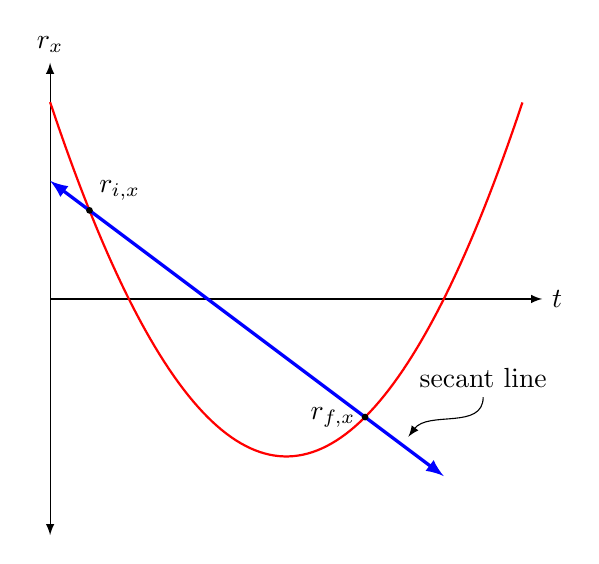
\begin{tikzpicture}[> = latex]

	% Graph axes
	
	\draw [<->] (0, -3) -- (0, 3) node [above] {$r_x$};
	\draw [->] (0, 0) -- (6.25, 0) node [right] {$t$};
	
	% Graph curve
	
	\draw [red, thick] plot [variable = \t, domain = 0 : 6, samples = 100] ({\t}, {0.5 * (\t - 3)^2 - 2});
	
	% Secant line
	
	\draw [very thick, blue, <->] (0, 1.5) -- (5, -2.25);
	\draw [fill = black] (0.5, 1.125) circle (1 pt) node [above right] {$r_{i, x}$};
	\draw [fill = black] (4, -1.5) circle (1 pt) node [left] {$r_{f, x}$};
	
	\node (secant) at (5.5, -1) {secant line};
	\draw [->] (secant.south) to [out = 270, in = 53.1] (4.55, -1.75);
	
\end{tikzpicture}
\end{document}